% Created by tikzDevice version 0.12.4 on 2023-09-13 23:40:03
% !TEX encoding = UTF-8 Unicode
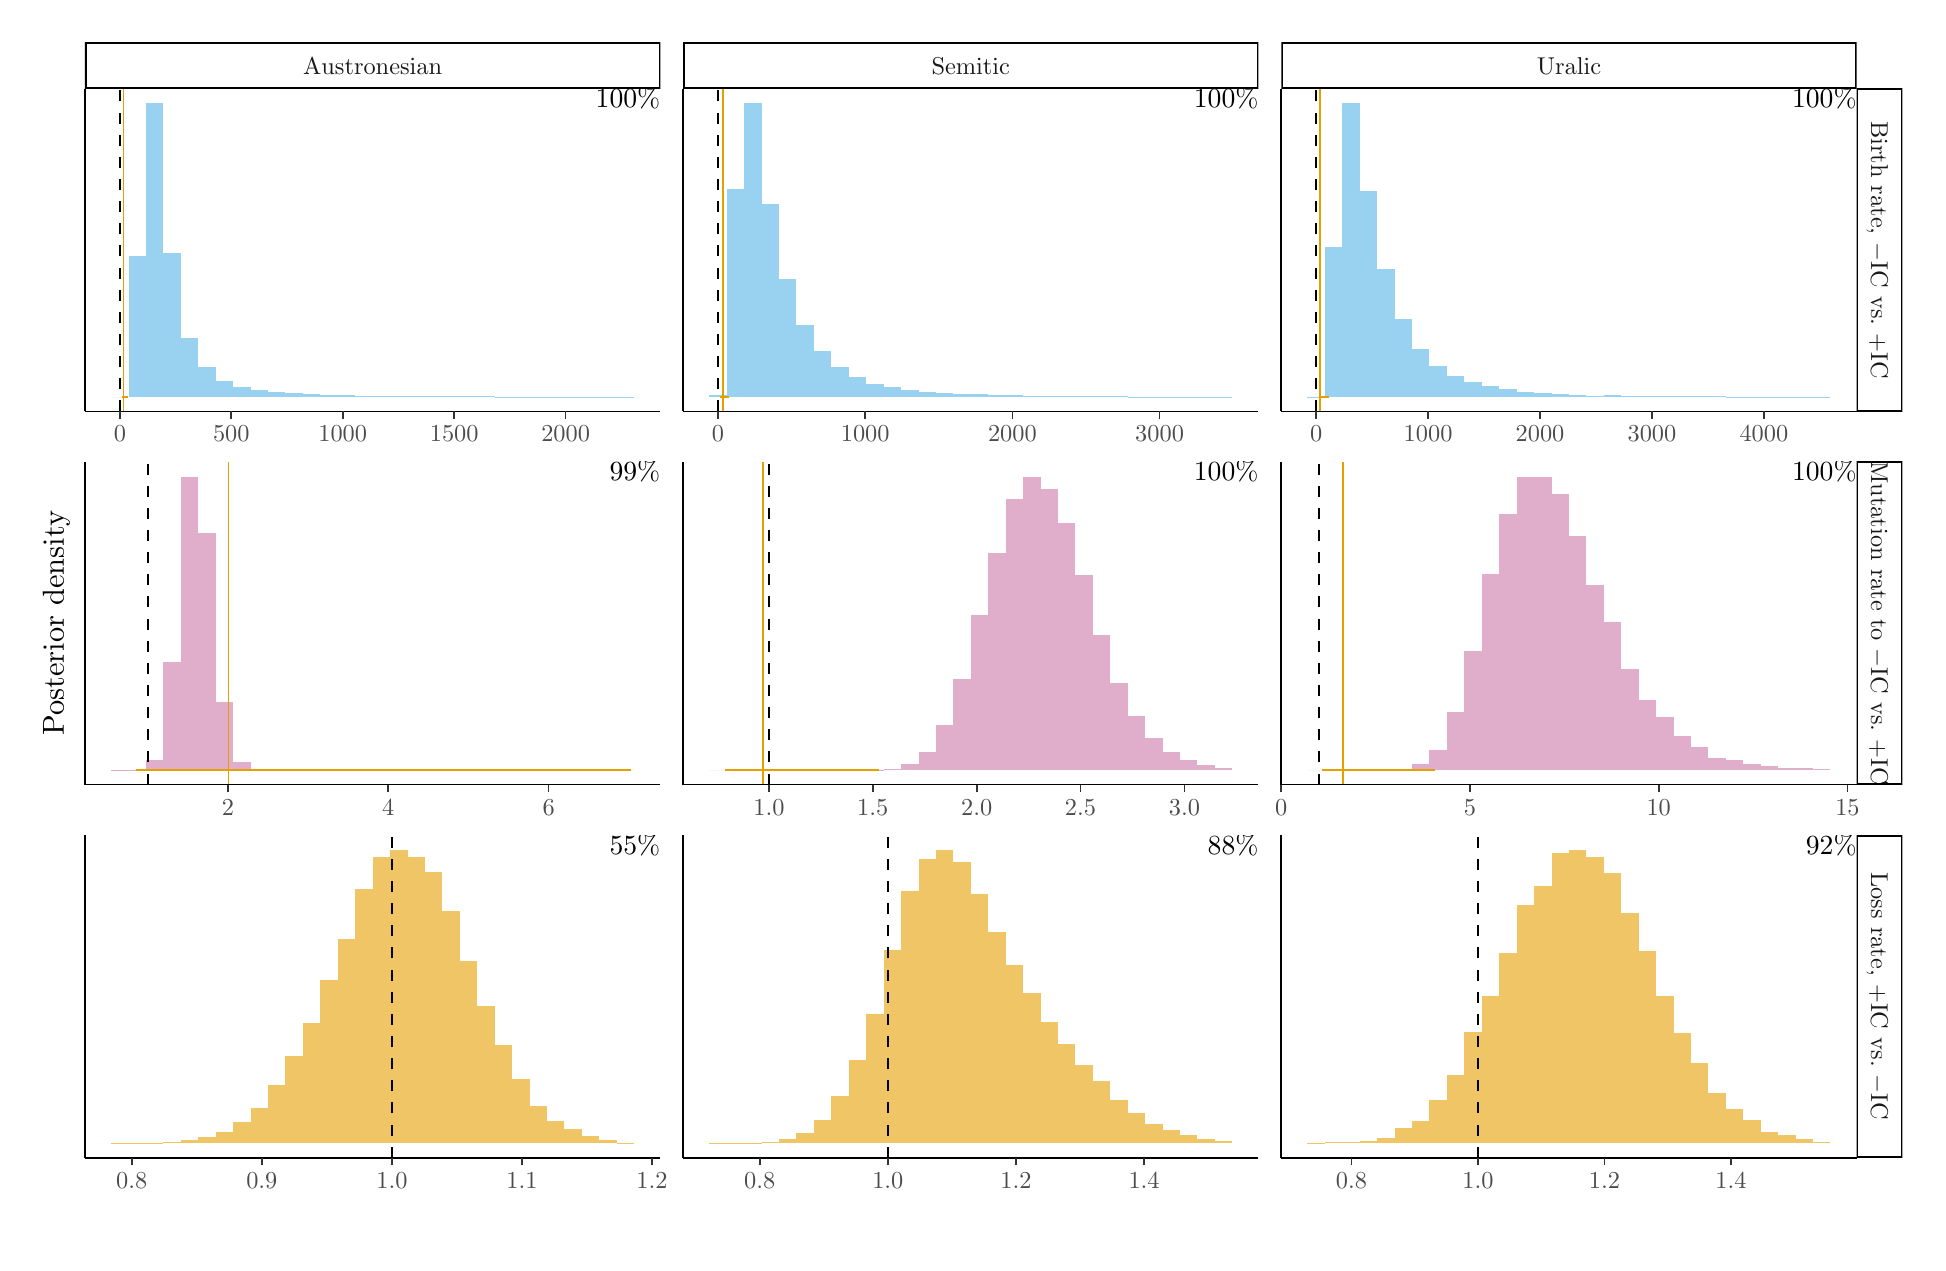
\begin{tikzpicture}[x=1pt,y=1pt]
\definecolor{fillColor}{RGB}{255,255,255}
\path[use as bounding box,fill=fillColor,fill opacity=0.00] (0,0) rectangle (682.95,439.04);
\begin{scope}
\path[clip] (  0.00,  0.00) rectangle (682.95,439.04);
\definecolor{drawColor}{RGB}{255,255,255}
\definecolor{fillColor}{RGB}{255,255,255}

\path[draw=drawColor,line width= 0.6pt,line join=round,line cap=round,fill=fillColor] (  0.00,  0.00) rectangle (682.95,439.04);
\end{scope}
\begin{scope}
\path[clip] ( 20.71,300.36) rectangle (228.60,416.97);
\definecolor{fillColor}{RGB}{255,255,255}

\path[fill=fillColor] ( 20.71,300.36) rectangle (228.60,416.97);
\definecolor{fillColor}{RGB}{86,180,233}

\path[fill=fillColor,fill opacity=0.60] ( 30.16,305.66) rectangle ( 36.46,305.66);

\path[fill=fillColor,fill opacity=0.60] ( 36.46,305.66) rectangle ( 42.76,356.58);

\path[fill=fillColor,fill opacity=0.60] ( 42.76,305.66) rectangle ( 49.06,411.67);

\path[fill=fillColor,fill opacity=0.60] ( 49.06,305.66) rectangle ( 55.36,357.50);

\path[fill=fillColor,fill opacity=0.60] ( 55.36,305.66) rectangle ( 61.66,327.04);

\path[fill=fillColor,fill opacity=0.60] ( 61.66,305.66) rectangle ( 67.96,316.33);

\path[fill=fillColor,fill opacity=0.60] ( 67.96,305.66) rectangle ( 74.26,311.29);

\path[fill=fillColor,fill opacity=0.60] ( 74.26,305.66) rectangle ( 80.56,309.32);

\path[fill=fillColor,fill opacity=0.60] ( 80.56,305.66) rectangle ( 86.86,308.14);

\path[fill=fillColor,fill opacity=0.60] ( 86.86,305.66) rectangle ( 93.16,307.30);

\path[fill=fillColor,fill opacity=0.60] ( 93.16,305.66) rectangle ( 99.46,306.94);

\path[fill=fillColor,fill opacity=0.60] ( 99.46,305.66) rectangle (105.76,306.60);

\path[fill=fillColor,fill opacity=0.60] (105.76,305.66) rectangle (112.06,306.36);

\path[fill=fillColor,fill opacity=0.60] (112.06,305.66) rectangle (118.36,306.21);

\path[fill=fillColor,fill opacity=0.60] (118.36,305.66) rectangle (124.66,306.10);

\path[fill=fillColor,fill opacity=0.60] (124.66,305.66) rectangle (130.96,305.99);

\path[fill=fillColor,fill opacity=0.60] (130.96,305.66) rectangle (137.26,305.93);

\path[fill=fillColor,fill opacity=0.60] (137.26,305.66) rectangle (143.56,305.89);

\path[fill=fillColor,fill opacity=0.60] (143.56,305.66) rectangle (149.86,305.90);

\path[fill=fillColor,fill opacity=0.60] (149.86,305.66) rectangle (156.16,305.81);

\path[fill=fillColor,fill opacity=0.60] (156.16,305.66) rectangle (162.46,305.80);

\path[fill=fillColor,fill opacity=0.60] (162.46,305.66) rectangle (168.76,305.78);

\path[fill=fillColor,fill opacity=0.60] (168.76,305.66) rectangle (175.06,305.73);

\path[fill=fillColor,fill opacity=0.60] (175.06,305.66) rectangle (181.36,305.71);

\path[fill=fillColor,fill opacity=0.60] (181.36,305.66) rectangle (187.66,305.72);

\path[fill=fillColor,fill opacity=0.60] (187.66,305.66) rectangle (193.95,305.69);

\path[fill=fillColor,fill opacity=0.60] (193.95,305.66) rectangle (200.25,305.70);

\path[fill=fillColor,fill opacity=0.60] (200.25,305.66) rectangle (206.55,305.69);

\path[fill=fillColor,fill opacity=0.60] (206.55,305.66) rectangle (212.85,305.68);

\path[fill=fillColor,fill opacity=0.60] (212.85,305.66) rectangle (219.15,305.68);
\definecolor{drawColor}{RGB}{0,0,0}

\path[draw=drawColor,line width= 0.6pt,dash pattern=on 4pt off 4pt ,line join=round] ( 33.39,300.36) -- ( 33.39,416.97);
\definecolor{drawColor}{RGB}{230,159,0}

\path[draw=drawColor,line width= 0.6pt,line join=round] ( 34.68,300.36) -- ( 34.68,416.97);

\path[draw=drawColor,line width= 0.6pt,line join=round] ( 33.96,305.66) --
	( 36.29,305.66);
\definecolor{drawColor}{RGB}{0,0,0}

\node[text=drawColor,anchor=base east,inner sep=0pt, outer sep=0pt, scale=  1.00] at (228.60,410.11) {100\%};
\end{scope}
\begin{scope}
\path[clip] (236.85,300.36) rectangle (444.74,416.97);
\definecolor{fillColor}{RGB}{255,255,255}

\path[fill=fillColor] (236.85,300.36) rectangle (444.74,416.97);
\definecolor{fillColor}{RGB}{86,180,233}

\path[fill=fillColor,fill opacity=0.60] (246.30,305.66) rectangle (252.60,306.23);

\path[fill=fillColor,fill opacity=0.60] (252.60,305.66) rectangle (258.90,380.86);

\path[fill=fillColor,fill opacity=0.60] (258.90,305.66) rectangle (265.20,411.67);

\path[fill=fillColor,fill opacity=0.60] (265.20,305.66) rectangle (271.50,375.35);

\path[fill=fillColor,fill opacity=0.60] (271.50,305.66) rectangle (277.80,348.30);

\path[fill=fillColor,fill opacity=0.60] (277.80,305.66) rectangle (284.10,331.73);

\path[fill=fillColor,fill opacity=0.60] (284.10,305.66) rectangle (290.40,322.31);

\path[fill=fillColor,fill opacity=0.60] (290.40,305.66) rectangle (296.70,316.29);

\path[fill=fillColor,fill opacity=0.60] (296.70,305.66) rectangle (303.00,312.65);

\path[fill=fillColor,fill opacity=0.60] (303.00,305.66) rectangle (309.30,310.45);

\path[fill=fillColor,fill opacity=0.60] (309.30,305.66) rectangle (315.60,309.08);

\path[fill=fillColor,fill opacity=0.60] (315.60,305.66) rectangle (321.90,308.11);

\path[fill=fillColor,fill opacity=0.60] (321.90,305.66) rectangle (328.20,307.36);

\path[fill=fillColor,fill opacity=0.60] (328.20,305.66) rectangle (334.50,306.92);

\path[fill=fillColor,fill opacity=0.60] (334.50,305.66) rectangle (340.80,306.67);

\path[fill=fillColor,fill opacity=0.60] (340.80,305.66) rectangle (347.10,306.59);

\path[fill=fillColor,fill opacity=0.60] (347.10,305.66) rectangle (353.40,306.21);

\path[fill=fillColor,fill opacity=0.60] (353.40,305.66) rectangle (359.70,306.15);

\path[fill=fillColor,fill opacity=0.60] (359.70,305.66) rectangle (366.00,306.02);

\path[fill=fillColor,fill opacity=0.60] (366.00,305.66) rectangle (372.30,306.00);

\path[fill=fillColor,fill opacity=0.60] (372.30,305.66) rectangle (378.60,305.94);

\path[fill=fillColor,fill opacity=0.60] (378.60,305.66) rectangle (384.89,305.88);

\path[fill=fillColor,fill opacity=0.60] (384.89,305.66) rectangle (391.19,305.83);

\path[fill=fillColor,fill opacity=0.60] (391.19,305.66) rectangle (397.49,305.83);

\path[fill=fillColor,fill opacity=0.60] (397.49,305.66) rectangle (403.79,305.74);

\path[fill=fillColor,fill opacity=0.60] (403.79,305.66) rectangle (410.09,305.76);

\path[fill=fillColor,fill opacity=0.60] (410.09,305.66) rectangle (416.39,305.72);

\path[fill=fillColor,fill opacity=0.60] (416.39,305.66) rectangle (422.69,305.75);

\path[fill=fillColor,fill opacity=0.60] (422.69,305.66) rectangle (428.99,305.73);

\path[fill=fillColor,fill opacity=0.60] (428.99,305.66) rectangle (435.29,305.67);
\definecolor{drawColor}{RGB}{0,0,0}

\path[draw=drawColor,line width= 0.6pt,dash pattern=on 4pt off 4pt ,line join=round] (249.51,300.36) -- (249.51,416.97);
\definecolor{drawColor}{RGB}{230,159,0}

\path[draw=drawColor,line width= 0.6pt,line join=round] (251.15,300.36) -- (251.15,416.97);

\path[draw=drawColor,line width= 0.6pt,line join=round] (250.30,305.66) --
	(253.33,305.66);
\definecolor{drawColor}{RGB}{0,0,0}

\node[text=drawColor,anchor=base east,inner sep=0pt, outer sep=0pt, scale=  1.00] at (444.74,410.11) {100\%};
\end{scope}
\begin{scope}
\path[clip] (452.99,300.36) rectangle (660.88,416.97);
\definecolor{fillColor}{RGB}{255,255,255}

\path[fill=fillColor] (452.99,300.36) rectangle (660.88,416.97);
\definecolor{fillColor}{RGB}{86,180,233}

\path[fill=fillColor,fill opacity=0.60] (462.44,305.66) rectangle (468.74,305.71);

\path[fill=fillColor,fill opacity=0.60] (468.74,305.66) rectangle (475.04,359.76);

\path[fill=fillColor,fill opacity=0.60] (475.04,305.66) rectangle (481.34,411.67);

\path[fill=fillColor,fill opacity=0.60] (481.34,305.66) rectangle (487.64,380.17);

\path[fill=fillColor,fill opacity=0.60] (487.64,305.66) rectangle (493.94,351.80);

\path[fill=fillColor,fill opacity=0.60] (493.94,305.66) rectangle (500.24,333.70);

\path[fill=fillColor,fill opacity=0.60] (500.24,305.66) rectangle (506.54,322.88);

\path[fill=fillColor,fill opacity=0.60] (506.54,305.66) rectangle (512.84,316.83);

\path[fill=fillColor,fill opacity=0.60] (512.84,305.66) rectangle (519.14,313.04);

\path[fill=fillColor,fill opacity=0.60] (519.14,305.66) rectangle (525.44,310.87);

\path[fill=fillColor,fill opacity=0.60] (525.44,305.66) rectangle (531.74,309.42);

\path[fill=fillColor,fill opacity=0.60] (531.74,305.66) rectangle (538.04,308.32);

\path[fill=fillColor,fill opacity=0.60] (538.04,305.66) rectangle (544.34,307.56);

\path[fill=fillColor,fill opacity=0.60] (544.34,305.66) rectangle (550.64,307.01);

\path[fill=fillColor,fill opacity=0.60] (550.64,305.66) rectangle (556.94,306.77);

\path[fill=fillColor,fill opacity=0.60] (556.94,305.66) rectangle (563.24,306.34);

\path[fill=fillColor,fill opacity=0.60] (563.24,305.66) rectangle (569.54,306.08);

\path[fill=fillColor,fill opacity=0.60] (569.54,305.66) rectangle (575.83,306.25);

\path[fill=fillColor,fill opacity=0.60] (575.83,305.66) rectangle (582.13,306.02);

\path[fill=fillColor,fill opacity=0.60] (582.13,305.66) rectangle (588.43,306.02);

\path[fill=fillColor,fill opacity=0.60] (588.43,305.66) rectangle (594.73,305.86);

\path[fill=fillColor,fill opacity=0.60] (594.73,305.66) rectangle (601.03,305.85);

\path[fill=fillColor,fill opacity=0.60] (601.03,305.66) rectangle (607.33,305.78);

\path[fill=fillColor,fill opacity=0.60] (607.33,305.66) rectangle (613.63,305.81);

\path[fill=fillColor,fill opacity=0.60] (613.63,305.66) rectangle (619.93,305.75);

\path[fill=fillColor,fill opacity=0.60] (619.93,305.66) rectangle (626.23,305.71);

\path[fill=fillColor,fill opacity=0.60] (626.23,305.66) rectangle (632.53,305.71);

\path[fill=fillColor,fill opacity=0.60] (632.53,305.66) rectangle (638.83,305.71);

\path[fill=fillColor,fill opacity=0.60] (638.83,305.66) rectangle (645.13,305.71);

\path[fill=fillColor,fill opacity=0.60] (645.13,305.66) rectangle (651.43,305.67);
\definecolor{drawColor}{RGB}{0,0,0}

\path[draw=drawColor,line width= 0.6pt,dash pattern=on 4pt off 4pt ,line join=round] (465.63,300.36) -- (465.63,416.97);
\definecolor{drawColor}{RGB}{230,159,0}

\path[draw=drawColor,line width= 0.6pt,line join=round] (467.03,300.36) -- (467.03,416.97);

\path[draw=drawColor,line width= 0.6pt,line join=round] (466.44,305.66) --
	(470.12,305.66);
\definecolor{drawColor}{RGB}{0,0,0}

\node[text=drawColor,anchor=base east,inner sep=0pt, outer sep=0pt, scale=  1.00] at (660.88,410.11) {100\%};
\end{scope}
\begin{scope}
\path[clip] ( 20.71,165.52) rectangle (228.60,282.13);
\definecolor{fillColor}{RGB}{255,255,255}

\path[fill=fillColor] ( 20.71,165.52) rectangle (228.60,282.13);
\definecolor{fillColor}{RGB}{204,121,167}

\path[fill=fillColor,fill opacity=0.60] ( 30.16,170.82) rectangle ( 36.46,170.83);

\path[fill=fillColor,fill opacity=0.60] ( 36.46,170.82) rectangle ( 42.76,170.91);

\path[fill=fillColor,fill opacity=0.60] ( 42.76,170.82) rectangle ( 49.06,174.36);

\path[fill=fillColor,fill opacity=0.60] ( 49.06,170.82) rectangle ( 55.36,209.73);

\path[fill=fillColor,fill opacity=0.60] ( 55.36,170.82) rectangle ( 61.66,276.83);

\path[fill=fillColor,fill opacity=0.60] ( 61.66,170.82) rectangle ( 67.96,256.57);

\path[fill=fillColor,fill opacity=0.60] ( 67.96,170.82) rectangle ( 74.26,195.49);

\path[fill=fillColor,fill opacity=0.60] ( 74.26,170.82) rectangle ( 80.56,173.79);

\path[fill=fillColor,fill opacity=0.60] ( 80.56,170.82) rectangle ( 86.86,170.82);

\path[fill=fillColor,fill opacity=0.60] ( 86.86,170.82) rectangle ( 93.16,170.82);

\path[fill=fillColor,fill opacity=0.60] ( 93.16,170.82) rectangle ( 99.46,170.82);

\path[fill=fillColor,fill opacity=0.60] ( 99.46,170.82) rectangle (105.76,170.82);

\path[fill=fillColor,fill opacity=0.60] (105.76,170.82) rectangle (112.06,170.82);

\path[fill=fillColor,fill opacity=0.60] (112.06,170.82) rectangle (118.36,170.82);

\path[fill=fillColor,fill opacity=0.60] (118.36,170.82) rectangle (124.66,170.82);

\path[fill=fillColor,fill opacity=0.60] (124.66,170.82) rectangle (130.96,170.82);

\path[fill=fillColor,fill opacity=0.60] (130.96,170.82) rectangle (137.26,170.82);

\path[fill=fillColor,fill opacity=0.60] (137.26,170.82) rectangle (143.56,170.82);

\path[fill=fillColor,fill opacity=0.60] (143.56,170.82) rectangle (149.86,170.82);

\path[fill=fillColor,fill opacity=0.60] (149.86,170.82) rectangle (156.16,170.82);

\path[fill=fillColor,fill opacity=0.60] (156.16,170.82) rectangle (162.46,170.82);

\path[fill=fillColor,fill opacity=0.60] (162.46,170.82) rectangle (168.76,170.82);

\path[fill=fillColor,fill opacity=0.60] (168.76,170.82) rectangle (175.06,170.82);

\path[fill=fillColor,fill opacity=0.60] (175.06,170.82) rectangle (181.36,170.82);

\path[fill=fillColor,fill opacity=0.60] (181.36,170.82) rectangle (187.66,170.82);

\path[fill=fillColor,fill opacity=0.60] (187.66,170.82) rectangle (193.95,170.82);

\path[fill=fillColor,fill opacity=0.60] (193.95,170.82) rectangle (200.25,170.82);

\path[fill=fillColor,fill opacity=0.60] (200.25,170.82) rectangle (206.55,170.82);

\path[fill=fillColor,fill opacity=0.60] (206.55,170.82) rectangle (212.85,170.82);

\path[fill=fillColor,fill opacity=0.60] (212.85,170.82) rectangle (219.15,170.82);
\definecolor{drawColor}{RGB}{0,0,0}

\path[draw=drawColor,line width= 0.6pt,dash pattern=on 4pt off 4pt ,line join=round] ( 43.39,165.52) -- ( 43.39,282.13);
\definecolor{drawColor}{RGB}{230,159,0}

\path[draw=drawColor,line width= 0.6pt,line join=round] ( 72.58,165.52) -- ( 72.58,282.13);

\path[draw=drawColor,line width= 0.6pt,line join=round] ( 39.18,170.82) --
	(217.93,170.82);
\definecolor{drawColor}{RGB}{0,0,0}

\node[text=drawColor,anchor=base east,inner sep=0pt, outer sep=0pt, scale=  1.00] at (228.60,275.28) {99\%};
\end{scope}
\begin{scope}
\path[clip] (236.85,165.52) rectangle (444.74,282.13);
\definecolor{fillColor}{RGB}{255,255,255}

\path[fill=fillColor] (236.85,165.52) rectangle (444.74,282.13);
\definecolor{fillColor}{RGB}{204,121,167}

\path[fill=fillColor,fill opacity=0.60] (246.30,170.82) rectangle (252.60,170.82);

\path[fill=fillColor,fill opacity=0.60] (252.60,170.82) rectangle (258.90,170.82);

\path[fill=fillColor,fill opacity=0.60] (258.90,170.82) rectangle (265.20,170.82);

\path[fill=fillColor,fill opacity=0.60] (265.20,170.82) rectangle (271.50,170.82);

\path[fill=fillColor,fill opacity=0.60] (271.50,170.82) rectangle (277.80,170.82);

\path[fill=fillColor,fill opacity=0.60] (277.80,170.82) rectangle (284.10,170.82);

\path[fill=fillColor,fill opacity=0.60] (284.10,170.82) rectangle (290.40,170.82);

\path[fill=fillColor,fill opacity=0.60] (290.40,170.82) rectangle (296.70,170.82);

\path[fill=fillColor,fill opacity=0.60] (296.70,170.82) rectangle (303.00,170.83);

\path[fill=fillColor,fill opacity=0.60] (303.00,170.82) rectangle (309.30,170.93);

\path[fill=fillColor,fill opacity=0.60] (309.30,170.82) rectangle (315.60,171.31);

\path[fill=fillColor,fill opacity=0.60] (315.60,170.82) rectangle (321.90,173.04);

\path[fill=fillColor,fill opacity=0.60] (321.90,170.82) rectangle (328.20,177.24);

\path[fill=fillColor,fill opacity=0.60] (328.20,170.82) rectangle (334.50,186.92);

\path[fill=fillColor,fill opacity=0.60] (334.50,170.82) rectangle (340.80,203.82);

\path[fill=fillColor,fill opacity=0.60] (340.80,170.82) rectangle (347.10,226.91);

\path[fill=fillColor,fill opacity=0.60] (347.10,170.82) rectangle (353.40,249.30);

\path[fill=fillColor,fill opacity=0.60] (353.40,170.82) rectangle (359.70,268.73);

\path[fill=fillColor,fill opacity=0.60] (359.70,170.82) rectangle (366.00,276.83);

\path[fill=fillColor,fill opacity=0.60] (366.00,170.82) rectangle (372.30,272.39);

\path[fill=fillColor,fill opacity=0.60] (372.30,170.82) rectangle (378.60,260.21);

\path[fill=fillColor,fill opacity=0.60] (378.60,170.82) rectangle (384.89,241.13);

\path[fill=fillColor,fill opacity=0.60] (384.89,170.82) rectangle (391.19,219.64);

\path[fill=fillColor,fill opacity=0.60] (391.19,170.82) rectangle (397.49,202.21);

\path[fill=fillColor,fill opacity=0.60] (397.49,170.82) rectangle (403.79,190.31);

\path[fill=fillColor,fill opacity=0.60] (403.79,170.82) rectangle (410.09,182.42);

\path[fill=fillColor,fill opacity=0.60] (410.09,170.82) rectangle (416.39,177.15);

\path[fill=fillColor,fill opacity=0.60] (416.39,170.82) rectangle (422.69,174.39);

\path[fill=fillColor,fill opacity=0.60] (422.69,170.82) rectangle (428.99,172.49);

\path[fill=fillColor,fill opacity=0.60] (428.99,170.82) rectangle (435.29,171.66);
\definecolor{drawColor}{RGB}{0,0,0}

\path[draw=drawColor,line width= 0.6pt,dash pattern=on 4pt off 4pt ,line join=round] (267.84,165.52) -- (267.84,282.13);
\definecolor{drawColor}{RGB}{230,159,0}

\path[draw=drawColor,line width= 0.6pt,line join=round] (265.73,165.52) -- (265.73,282.13);

\path[draw=drawColor,line width= 0.6pt,line join=round] (252.05,170.82) --
	(307.57,170.82);
\definecolor{drawColor}{RGB}{0,0,0}

\node[text=drawColor,anchor=base east,inner sep=0pt, outer sep=0pt, scale=  1.00] at (444.74,275.28) {100\%};
\end{scope}
\begin{scope}
\path[clip] (452.99,165.52) rectangle (660.88,282.13);
\definecolor{fillColor}{RGB}{255,255,255}

\path[fill=fillColor] (452.99,165.52) rectangle (660.88,282.13);
\definecolor{fillColor}{RGB}{204,121,167}

\path[fill=fillColor,fill opacity=0.60] (462.44,170.82) rectangle (468.74,170.82);

\path[fill=fillColor,fill opacity=0.60] (468.74,170.82) rectangle (475.04,170.82);

\path[fill=fillColor,fill opacity=0.60] (475.04,170.82) rectangle (481.34,170.82);

\path[fill=fillColor,fill opacity=0.60] (481.34,170.82) rectangle (487.64,170.82);

\path[fill=fillColor,fill opacity=0.60] (487.64,170.82) rectangle (493.94,170.86);

\path[fill=fillColor,fill opacity=0.60] (493.94,170.82) rectangle (500.24,171.06);

\path[fill=fillColor,fill opacity=0.60] (500.24,170.82) rectangle (506.54,172.89);

\path[fill=fillColor,fill opacity=0.60] (506.54,170.82) rectangle (512.84,178.11);

\path[fill=fillColor,fill opacity=0.60] (512.84,170.82) rectangle (519.14,191.74);

\path[fill=fillColor,fill opacity=0.60] (519.14,170.82) rectangle (525.44,213.70);

\path[fill=fillColor,fill opacity=0.60] (525.44,170.82) rectangle (531.74,241.64);

\path[fill=fillColor,fill opacity=0.60] (531.74,170.82) rectangle (538.04,263.48);

\path[fill=fillColor,fill opacity=0.60] (538.04,170.82) rectangle (544.34,276.83);

\path[fill=fillColor,fill opacity=0.60] (544.34,170.82) rectangle (550.64,276.68);

\path[fill=fillColor,fill opacity=0.60] (550.64,170.82) rectangle (556.94,270.41);

\path[fill=fillColor,fill opacity=0.60] (556.94,170.82) rectangle (563.24,255.29);

\path[fill=fillColor,fill opacity=0.60] (563.24,170.82) rectangle (569.54,237.77);

\path[fill=fillColor,fill opacity=0.60] (569.54,170.82) rectangle (575.83,224.22);

\path[fill=fillColor,fill opacity=0.60] (575.83,170.82) rectangle (582.13,207.12);

\path[fill=fillColor,fill opacity=0.60] (582.13,170.82) rectangle (588.43,196.26);

\path[fill=fillColor,fill opacity=0.60] (588.43,170.82) rectangle (594.73,190.12);

\path[fill=fillColor,fill opacity=0.60] (594.73,170.82) rectangle (601.03,183.12);

\path[fill=fillColor,fill opacity=0.60] (601.03,170.82) rectangle (607.33,179.12);

\path[fill=fillColor,fill opacity=0.60] (607.33,170.82) rectangle (613.63,175.13);

\path[fill=fillColor,fill opacity=0.60] (613.63,170.82) rectangle (619.93,174.42);

\path[fill=fillColor,fill opacity=0.60] (619.93,170.82) rectangle (626.23,172.95);

\path[fill=fillColor,fill opacity=0.60] (626.23,170.82) rectangle (632.53,172.26);

\path[fill=fillColor,fill opacity=0.60] (632.53,170.82) rectangle (638.83,171.67);

\path[fill=fillColor,fill opacity=0.60] (638.83,170.82) rectangle (645.13,171.41);

\path[fill=fillColor,fill opacity=0.60] (645.13,170.82) rectangle (651.43,171.18);
\definecolor{drawColor}{RGB}{0,0,0}

\path[draw=drawColor,line width= 0.6pt,dash pattern=on 4pt off 4pt ,line join=round] (466.63,165.52) -- (466.63,282.13);
\definecolor{drawColor}{RGB}{230,159,0}

\path[draw=drawColor,line width= 0.6pt,line join=round] (475.29,165.52) -- (475.29,282.13);

\path[draw=drawColor,line width= 0.6pt,line join=round] (467.72,170.82) --
	(508.41,170.82);
\definecolor{drawColor}{RGB}{0,0,0}

\node[text=drawColor,anchor=base east,inner sep=0pt, outer sep=0pt, scale=  1.00] at (660.88,275.28) {100\%};
\end{scope}
\begin{scope}
\path[clip] ( 20.71, 30.69) rectangle (228.60,147.30);
\definecolor{fillColor}{RGB}{255,255,255}

\path[fill=fillColor] ( 20.71, 30.69) rectangle (228.60,147.30);
\definecolor{fillColor}{RGB}{230,159,0}

\path[fill=fillColor,fill opacity=0.60] ( 30.16, 35.99) rectangle ( 36.46, 36.05);

\path[fill=fillColor,fill opacity=0.60] ( 36.46, 35.99) rectangle ( 42.76, 36.09);

\path[fill=fillColor,fill opacity=0.60] ( 42.76, 35.99) rectangle ( 49.06, 36.14);

\path[fill=fillColor,fill opacity=0.60] ( 49.06, 35.99) rectangle ( 55.36, 36.39);

\path[fill=fillColor,fill opacity=0.60] ( 55.36, 35.99) rectangle ( 61.66, 36.94);

\path[fill=fillColor,fill opacity=0.60] ( 61.66, 35.99) rectangle ( 67.96, 38.13);

\path[fill=fillColor,fill opacity=0.60] ( 67.96, 35.99) rectangle ( 74.26, 39.90);

\path[fill=fillColor,fill opacity=0.60] ( 74.26, 35.99) rectangle ( 80.56, 43.67);

\path[fill=fillColor,fill opacity=0.60] ( 80.56, 35.99) rectangle ( 86.86, 48.84);

\path[fill=fillColor,fill opacity=0.60] ( 86.86, 35.99) rectangle ( 93.16, 56.86);

\path[fill=fillColor,fill opacity=0.60] ( 93.16, 35.99) rectangle ( 99.46, 67.28);

\path[fill=fillColor,fill opacity=0.60] ( 99.46, 35.99) rectangle (105.76, 79.37);

\path[fill=fillColor,fill opacity=0.60] (105.76, 35.99) rectangle (112.06, 95.07);

\path[fill=fillColor,fill opacity=0.60] (112.06, 35.99) rectangle (118.36,109.74);

\path[fill=fillColor,fill opacity=0.60] (118.36, 35.99) rectangle (124.66,127.62);

\path[fill=fillColor,fill opacity=0.60] (124.66, 35.99) rectangle (130.96,139.36);

\path[fill=fillColor,fill opacity=0.60] (130.96, 35.99) rectangle (137.26,142.00);

\path[fill=fillColor,fill opacity=0.60] (137.26, 35.99) rectangle (143.56,139.23);

\path[fill=fillColor,fill opacity=0.60] (143.56, 35.99) rectangle (149.86,134.05);

\path[fill=fillColor,fill opacity=0.60] (149.86, 35.99) rectangle (156.16,119.97);

\path[fill=fillColor,fill opacity=0.60] (156.16, 35.99) rectangle (162.46,101.66);

\path[fill=fillColor,fill opacity=0.60] (162.46, 35.99) rectangle (168.76, 85.47);

\path[fill=fillColor,fill opacity=0.60] (168.76, 35.99) rectangle (175.06, 71.31);

\path[fill=fillColor,fill opacity=0.60] (175.06, 35.99) rectangle (181.36, 59.05);

\path[fill=fillColor,fill opacity=0.60] (181.36, 35.99) rectangle (187.66, 49.21);

\path[fill=fillColor,fill opacity=0.60] (187.66, 35.99) rectangle (193.95, 43.92);

\path[fill=fillColor,fill opacity=0.60] (193.95, 35.99) rectangle (200.25, 40.98);

\path[fill=fillColor,fill opacity=0.60] (200.25, 35.99) rectangle (206.55, 38.53);

\path[fill=fillColor,fill opacity=0.60] (206.55, 35.99) rectangle (212.85, 37.28);

\path[fill=fillColor,fill opacity=0.60] (212.85, 35.99) rectangle (219.15, 36.08);
\definecolor{drawColor}{RGB}{0,0,0}

\path[draw=drawColor,line width= 0.6pt,dash pattern=on 4pt off 4pt ,line join=round] (131.62, 30.69) -- (131.62,147.30);

\node[text=drawColor,anchor=base east,inner sep=0pt, outer sep=0pt, scale=  1.00] at (228.60,140.44) {55\%};
\end{scope}
\begin{scope}
\path[clip] (236.85, 30.69) rectangle (444.74,147.30);
\definecolor{fillColor}{RGB}{255,255,255}

\path[fill=fillColor] (236.85, 30.69) rectangle (444.74,147.30);
\definecolor{fillColor}{RGB}{230,159,0}

\path[fill=fillColor,fill opacity=0.60] (246.30, 35.99) rectangle (252.60, 36.00);

\path[fill=fillColor,fill opacity=0.60] (252.60, 35.99) rectangle (258.90, 36.03);

\path[fill=fillColor,fill opacity=0.60] (258.90, 35.99) rectangle (265.20, 36.18);

\path[fill=fillColor,fill opacity=0.60] (265.20, 35.99) rectangle (271.50, 36.45);

\path[fill=fillColor,fill opacity=0.60] (271.50, 35.99) rectangle (277.80, 37.45);

\path[fill=fillColor,fill opacity=0.60] (277.80, 35.99) rectangle (284.10, 39.53);

\path[fill=fillColor,fill opacity=0.60] (284.10, 35.99) rectangle (290.40, 44.38);

\path[fill=fillColor,fill opacity=0.60] (290.40, 35.99) rectangle (296.70, 53.11);

\path[fill=fillColor,fill opacity=0.60] (296.70, 35.99) rectangle (303.00, 65.90);

\path[fill=fillColor,fill opacity=0.60] (303.00, 35.99) rectangle (309.30, 82.76);

\path[fill=fillColor,fill opacity=0.60] (309.30, 35.99) rectangle (315.60,105.93);

\path[fill=fillColor,fill opacity=0.60] (315.60, 35.99) rectangle (321.90,126.96);

\path[fill=fillColor,fill opacity=0.60] (321.90, 35.99) rectangle (328.20,138.50);

\path[fill=fillColor,fill opacity=0.60] (328.20, 35.99) rectangle (334.50,142.00);

\path[fill=fillColor,fill opacity=0.60] (334.50, 35.99) rectangle (340.80,137.38);

\path[fill=fillColor,fill opacity=0.60] (340.80, 35.99) rectangle (347.10,125.99);

\path[fill=fillColor,fill opacity=0.60] (347.10, 35.99) rectangle (353.40,112.21);

\path[fill=fillColor,fill opacity=0.60] (353.40, 35.99) rectangle (359.70,100.37);

\path[fill=fillColor,fill opacity=0.60] (359.70, 35.99) rectangle (366.00, 90.24);

\path[fill=fillColor,fill opacity=0.60] (366.00, 35.99) rectangle (372.30, 79.86);

\path[fill=fillColor,fill opacity=0.60] (372.30, 35.99) rectangle (378.60, 71.83);

\path[fill=fillColor,fill opacity=0.60] (378.60, 35.99) rectangle (384.89, 64.10);

\path[fill=fillColor,fill opacity=0.60] (384.89, 35.99) rectangle (391.19, 58.43);

\path[fill=fillColor,fill opacity=0.60] (391.19, 35.99) rectangle (397.49, 51.57);

\path[fill=fillColor,fill opacity=0.60] (397.49, 35.99) rectangle (403.79, 46.78);

\path[fill=fillColor,fill opacity=0.60] (403.79, 35.99) rectangle (410.09, 42.94);

\path[fill=fillColor,fill opacity=0.60] (410.09, 35.99) rectangle (416.39, 40.83);

\path[fill=fillColor,fill opacity=0.60] (416.39, 35.99) rectangle (422.69, 38.76);

\path[fill=fillColor,fill opacity=0.60] (422.69, 35.99) rectangle (428.99, 37.40);

\path[fill=fillColor,fill opacity=0.60] (428.99, 35.99) rectangle (435.29, 36.75);
\definecolor{drawColor}{RGB}{0,0,0}

\path[draw=drawColor,line width= 0.6pt,dash pattern=on 4pt off 4pt ,line join=round] (310.83, 30.69) -- (310.83,147.30);

\node[text=drawColor,anchor=base east,inner sep=0pt, outer sep=0pt, scale=  1.00] at (444.74,140.44) {88\%};
\end{scope}
\begin{scope}
\path[clip] (452.99, 30.69) rectangle (660.88,147.30);
\definecolor{fillColor}{RGB}{255,255,255}

\path[fill=fillColor] (452.99, 30.69) rectangle (660.88,147.30);
\definecolor{fillColor}{RGB}{230,159,0}

\path[fill=fillColor,fill opacity=0.60] (462.44, 35.99) rectangle (468.74, 36.09);

\path[fill=fillColor,fill opacity=0.60] (468.74, 35.99) rectangle (475.04, 36.22);

\path[fill=fillColor,fill opacity=0.60] (475.04, 35.99) rectangle (481.34, 36.55);

\path[fill=fillColor,fill opacity=0.60] (481.34, 35.99) rectangle (487.64, 36.76);

\path[fill=fillColor,fill opacity=0.60] (487.64, 35.99) rectangle (493.94, 37.99);

\path[fill=fillColor,fill opacity=0.60] (493.94, 35.99) rectangle (500.24, 41.31);

\path[fill=fillColor,fill opacity=0.60] (500.24, 35.99) rectangle (506.54, 44.04);

\path[fill=fillColor,fill opacity=0.60] (506.54, 35.99) rectangle (512.84, 51.45);

\path[fill=fillColor,fill opacity=0.60] (512.84, 35.99) rectangle (519.14, 60.57);

\path[fill=fillColor,fill opacity=0.60] (519.14, 35.99) rectangle (525.44, 75.96);

\path[fill=fillColor,fill opacity=0.60] (525.44, 35.99) rectangle (531.74, 89.21);

\path[fill=fillColor,fill opacity=0.60] (531.74, 35.99) rectangle (538.04,104.58);

\path[fill=fillColor,fill opacity=0.60] (538.04, 35.99) rectangle (544.34,121.90);

\path[fill=fillColor,fill opacity=0.60] (544.34, 35.99) rectangle (550.64,128.80);

\path[fill=fillColor,fill opacity=0.60] (550.64, 35.99) rectangle (556.94,140.71);

\path[fill=fillColor,fill opacity=0.60] (556.94, 35.99) rectangle (563.24,142.00);

\path[fill=fillColor,fill opacity=0.60] (563.24, 35.99) rectangle (569.54,139.24);

\path[fill=fillColor,fill opacity=0.60] (569.54, 35.99) rectangle (575.83,133.45);

\path[fill=fillColor,fill opacity=0.60] (575.83, 35.99) rectangle (582.13,119.22);

\path[fill=fillColor,fill opacity=0.60] (582.13, 35.99) rectangle (588.43,105.35);

\path[fill=fillColor,fill opacity=0.60] (588.43, 35.99) rectangle (594.73, 88.98);

\path[fill=fillColor,fill opacity=0.60] (594.73, 35.99) rectangle (601.03, 75.62);

\path[fill=fillColor,fill opacity=0.60] (601.03, 35.99) rectangle (607.33, 64.94);

\path[fill=fillColor,fill opacity=0.60] (607.33, 35.99) rectangle (613.63, 53.95);

\path[fill=fillColor,fill opacity=0.60] (613.63, 35.99) rectangle (619.93, 48.44);

\path[fill=fillColor,fill opacity=0.60] (619.93, 35.99) rectangle (626.23, 44.43);

\path[fill=fillColor,fill opacity=0.60] (626.23, 35.99) rectangle (632.53, 40.08);

\path[fill=fillColor,fill opacity=0.60] (632.53, 35.99) rectangle (638.83, 38.97);

\path[fill=fillColor,fill opacity=0.60] (638.83, 35.99) rectangle (645.13, 37.58);

\path[fill=fillColor,fill opacity=0.60] (645.13, 35.99) rectangle (651.43, 36.50);
\definecolor{drawColor}{RGB}{0,0,0}

\path[draw=drawColor,line width= 0.6pt,dash pattern=on 4pt off 4pt ,line join=round] (524.04, 30.69) -- (524.04,147.30);

\node[text=drawColor,anchor=base east,inner sep=0pt, outer sep=0pt, scale=  1.00] at (660.88,140.44) {92\%};
\end{scope}
\begin{scope}
\path[clip] ( 20.71,416.97) rectangle (228.60,433.54);
\definecolor{drawColor}{RGB}{0,0,0}
\definecolor{fillColor}{RGB}{255,255,255}

\path[draw=drawColor,line width= 1.1pt,line join=round,line cap=round,fill=fillColor] ( 20.71,416.97) rectangle (228.60,433.54);
\definecolor{drawColor}{gray}{0.10}

\node[text=drawColor,anchor=base,inner sep=0pt, outer sep=0pt, scale=  0.88] at (124.66,422.22) {Austronesian};
\end{scope}
\begin{scope}
\path[clip] (236.85,416.97) rectangle (444.74,433.54);
\definecolor{drawColor}{RGB}{0,0,0}
\definecolor{fillColor}{RGB}{255,255,255}

\path[draw=drawColor,line width= 1.1pt,line join=round,line cap=round,fill=fillColor] (236.85,416.97) rectangle (444.74,433.54);
\definecolor{drawColor}{gray}{0.10}

\node[text=drawColor,anchor=base,inner sep=0pt, outer sep=0pt, scale=  0.88] at (340.80,422.22) {Semitic};
\end{scope}
\begin{scope}
\path[clip] (452.99,416.97) rectangle (660.88,433.54);
\definecolor{drawColor}{RGB}{0,0,0}
\definecolor{fillColor}{RGB}{255,255,255}

\path[draw=drawColor,line width= 1.1pt,line join=round,line cap=round,fill=fillColor] (452.99,416.97) rectangle (660.88,433.54);
\definecolor{drawColor}{gray}{0.10}

\node[text=drawColor,anchor=base,inner sep=0pt, outer sep=0pt, scale=  0.88] at (556.94,422.22) {Uralic};
\end{scope}
\begin{scope}
\path[clip] (660.88,300.36) rectangle (677.45,416.97);
\definecolor{drawColor}{RGB}{0,0,0}
\definecolor{fillColor}{RGB}{255,255,255}

\path[draw=drawColor,line width= 1.1pt,line join=round,line cap=round,fill=fillColor] (660.88,300.36) rectangle (677.45,416.97);
\definecolor{drawColor}{gray}{0.10}

\node[text=drawColor,rotate=-90.00,anchor=base,inner sep=0pt, outer sep=0pt, scale=  0.88] at (666.14,358.66) {Birth rate, $-$IC vs.\ $+$IC};
\end{scope}
\begin{scope}
\path[clip] (660.88,165.52) rectangle (677.45,282.13);
\definecolor{drawColor}{RGB}{0,0,0}
\definecolor{fillColor}{RGB}{255,255,255}

\path[draw=drawColor,line width= 1.1pt,line join=round,line cap=round,fill=fillColor] (660.88,165.52) rectangle (677.45,282.13);
\definecolor{drawColor}{gray}{0.10}

\node[text=drawColor,rotate=-90.00,anchor=base,inner sep=0pt, outer sep=0pt, scale=  0.88] at (666.14,223.83) {Mutation rate to $-$IC vs.\ $+$IC};
\end{scope}
\begin{scope}
\path[clip] (660.88, 30.69) rectangle (677.45,147.30);
\definecolor{drawColor}{RGB}{0,0,0}
\definecolor{fillColor}{RGB}{255,255,255}

\path[draw=drawColor,line width= 1.1pt,line join=round,line cap=round,fill=fillColor] (660.88, 30.69) rectangle (677.45,147.30);
\definecolor{drawColor}{gray}{0.10}

\node[text=drawColor,rotate=-90.00,anchor=base,inner sep=0pt, outer sep=0pt, scale=  0.88] at (666.14, 88.99) {Loss rate, $+$IC vs.\ $-$IC};
\end{scope}
\begin{scope}
\path[clip] (  0.00,  0.00) rectangle (682.95,439.04);
\definecolor{drawColor}{RGB}{0,0,0}

\path[draw=drawColor,line width= 0.6pt,line join=round] ( 20.71, 30.69) --
	(228.60, 30.69);
\end{scope}
\begin{scope}
\path[clip] (  0.00,  0.00) rectangle (682.95,439.04);
\definecolor{drawColor}{gray}{0.20}

\path[draw=drawColor,line width= 0.6pt,line join=round] ( 37.62, 27.94) --
	( 37.62, 30.69);

\path[draw=drawColor,line width= 0.6pt,line join=round] ( 84.62, 27.94) --
	( 84.62, 30.69);

\path[draw=drawColor,line width= 0.6pt,line join=round] (131.62, 27.94) --
	(131.62, 30.69);

\path[draw=drawColor,line width= 0.6pt,line join=round] (178.62, 27.94) --
	(178.62, 30.69);

\path[draw=drawColor,line width= 0.6pt,line join=round] (225.61, 27.94) --
	(225.61, 30.69);
\end{scope}
\begin{scope}
\path[clip] (  0.00,  0.00) rectangle (682.95,439.04);
\definecolor{drawColor}{gray}{0.30}

\node[text=drawColor,anchor=base,inner sep=0pt, outer sep=0pt, scale=  0.88] at ( 37.62, 19.68) {0.8};

\node[text=drawColor,anchor=base,inner sep=0pt, outer sep=0pt, scale=  0.88] at ( 84.62, 19.68) {0.9};

\node[text=drawColor,anchor=base,inner sep=0pt, outer sep=0pt, scale=  0.88] at (131.62, 19.68) {1.0};

\node[text=drawColor,anchor=base,inner sep=0pt, outer sep=0pt, scale=  0.88] at (178.62, 19.68) {1.1};

\node[text=drawColor,anchor=base,inner sep=0pt, outer sep=0pt, scale=  0.88] at (225.61, 19.68) {1.2};
\end{scope}
\begin{scope}
\path[clip] (  0.00,  0.00) rectangle (682.95,439.04);
\definecolor{drawColor}{RGB}{0,0,0}

\path[draw=drawColor,line width= 0.6pt,line join=round] (236.85, 30.69) --
	(444.74, 30.69);
\end{scope}
\begin{scope}
\path[clip] (  0.00,  0.00) rectangle (682.95,439.04);
\definecolor{drawColor}{gray}{0.20}

\path[draw=drawColor,line width= 0.6pt,line join=round] (264.54, 27.94) --
	(264.54, 30.69);

\path[draw=drawColor,line width= 0.6pt,line join=round] (310.83, 27.94) --
	(310.83, 30.69);

\path[draw=drawColor,line width= 0.6pt,line join=round] (357.13, 27.94) --
	(357.13, 30.69);

\path[draw=drawColor,line width= 0.6pt,line join=round] (403.42, 27.94) --
	(403.42, 30.69);
\end{scope}
\begin{scope}
\path[clip] (  0.00,  0.00) rectangle (682.95,439.04);
\definecolor{drawColor}{gray}{0.30}

\node[text=drawColor,anchor=base,inner sep=0pt, outer sep=0pt, scale=  0.88] at (264.54, 19.68) {0.8};

\node[text=drawColor,anchor=base,inner sep=0pt, outer sep=0pt, scale=  0.88] at (310.83, 19.68) {1.0};

\node[text=drawColor,anchor=base,inner sep=0pt, outer sep=0pt, scale=  0.88] at (357.13, 19.68) {1.2};

\node[text=drawColor,anchor=base,inner sep=0pt, outer sep=0pt, scale=  0.88] at (403.42, 19.68) {1.4};
\end{scope}
\begin{scope}
\path[clip] (  0.00,  0.00) rectangle (682.95,439.04);
\definecolor{drawColor}{RGB}{0,0,0}

\path[draw=drawColor,line width= 0.6pt,line join=round] (452.99, 30.69) --
	(660.88, 30.69);
\end{scope}
\begin{scope}
\path[clip] (  0.00,  0.00) rectangle (682.95,439.04);
\definecolor{drawColor}{gray}{0.20}

\path[draw=drawColor,line width= 0.6pt,line join=round] (478.33, 27.94) --
	(478.33, 30.69);

\path[draw=drawColor,line width= 0.6pt,line join=round] (524.04, 27.94) --
	(524.04, 30.69);

\path[draw=drawColor,line width= 0.6pt,line join=round] (569.75, 27.94) --
	(569.75, 30.69);

\path[draw=drawColor,line width= 0.6pt,line join=round] (615.46, 27.94) --
	(615.46, 30.69);
\end{scope}
\begin{scope}
\path[clip] (  0.00,  0.00) rectangle (682.95,439.04);
\definecolor{drawColor}{gray}{0.30}

\node[text=drawColor,anchor=base,inner sep=0pt, outer sep=0pt, scale=  0.88] at (478.33, 19.68) {0.8};

\node[text=drawColor,anchor=base,inner sep=0pt, outer sep=0pt, scale=  0.88] at (524.04, 19.68) {1.0};

\node[text=drawColor,anchor=base,inner sep=0pt, outer sep=0pt, scale=  0.88] at (569.75, 19.68) {1.2};

\node[text=drawColor,anchor=base,inner sep=0pt, outer sep=0pt, scale=  0.88] at (615.46, 19.68) {1.4};
\end{scope}
\begin{scope}
\path[clip] (  0.00,  0.00) rectangle (682.95,439.04);
\definecolor{drawColor}{RGB}{0,0,0}

\path[draw=drawColor,line width= 0.6pt,line join=round] ( 20.71,165.52) --
	(228.60,165.52);
\end{scope}
\begin{scope}
\path[clip] (  0.00,  0.00) rectangle (682.95,439.04);
\definecolor{drawColor}{gray}{0.20}

\path[draw=drawColor,line width= 0.6pt,line join=round] ( 72.36,162.77) --
	( 72.36,165.52);

\path[draw=drawColor,line width= 0.6pt,line join=round] (130.30,162.77) --
	(130.30,165.52);

\path[draw=drawColor,line width= 0.6pt,line join=round] (188.24,162.77) --
	(188.24,165.52);
\end{scope}
\begin{scope}
\path[clip] (  0.00,  0.00) rectangle (682.95,439.04);
\definecolor{drawColor}{gray}{0.30}

\node[text=drawColor,anchor=base,inner sep=0pt, outer sep=0pt, scale=  0.88] at ( 72.36,154.51) {2};

\node[text=drawColor,anchor=base,inner sep=0pt, outer sep=0pt, scale=  0.88] at (130.30,154.51) {4};

\node[text=drawColor,anchor=base,inner sep=0pt, outer sep=0pt, scale=  0.88] at (188.24,154.51) {6};
\end{scope}
\begin{scope}
\path[clip] (  0.00,  0.00) rectangle (682.95,439.04);
\definecolor{drawColor}{RGB}{0,0,0}

\path[draw=drawColor,line width= 0.6pt,line join=round] (236.85,165.52) --
	(444.74,165.52);
\end{scope}
\begin{scope}
\path[clip] (  0.00,  0.00) rectangle (682.95,439.04);
\definecolor{drawColor}{gray}{0.20}

\path[draw=drawColor,line width= 0.6pt,line join=round] (267.84,162.77) --
	(267.84,165.52);

\path[draw=drawColor,line width= 0.6pt,line join=round] (305.38,162.77) --
	(305.38,165.52);

\path[draw=drawColor,line width= 0.6pt,line join=round] (342.92,162.77) --
	(342.92,165.52);

\path[draw=drawColor,line width= 0.6pt,line join=round] (380.46,162.77) --
	(380.46,165.52);

\path[draw=drawColor,line width= 0.6pt,line join=round] (418.00,162.77) --
	(418.00,165.52);
\end{scope}
\begin{scope}
\path[clip] (  0.00,  0.00) rectangle (682.95,439.04);
\definecolor{drawColor}{gray}{0.30}

\node[text=drawColor,anchor=base,inner sep=0pt, outer sep=0pt, scale=  0.88] at (267.84,154.51) {1.0};

\node[text=drawColor,anchor=base,inner sep=0pt, outer sep=0pt, scale=  0.88] at (305.38,154.51) {1.5};

\node[text=drawColor,anchor=base,inner sep=0pt, outer sep=0pt, scale=  0.88] at (342.92,154.51) {2.0};

\node[text=drawColor,anchor=base,inner sep=0pt, outer sep=0pt, scale=  0.88] at (380.46,154.51) {2.5};

\node[text=drawColor,anchor=base,inner sep=0pt, outer sep=0pt, scale=  0.88] at (418.00,154.51) {3.0};
\end{scope}
\begin{scope}
\path[clip] (  0.00,  0.00) rectangle (682.95,439.04);
\definecolor{drawColor}{RGB}{0,0,0}

\path[draw=drawColor,line width= 0.6pt,line join=round] (452.99,165.52) --
	(660.88,165.52);
\end{scope}
\begin{scope}
\path[clip] (  0.00,  0.00) rectangle (682.95,439.04);
\definecolor{drawColor}{gray}{0.20}

\path[draw=drawColor,line width= 0.6pt,line join=round] (452.99,162.77) --
	(452.99,165.52);

\path[draw=drawColor,line width= 0.6pt,line join=round] (521.19,162.77) --
	(521.19,165.52);

\path[draw=drawColor,line width= 0.6pt,line join=round] (589.38,162.77) --
	(589.38,165.52);

\path[draw=drawColor,line width= 0.6pt,line join=round] (657.58,162.77) --
	(657.58,165.52);
\end{scope}
\begin{scope}
\path[clip] (  0.00,  0.00) rectangle (682.95,439.04);
\definecolor{drawColor}{gray}{0.30}

\node[text=drawColor,anchor=base,inner sep=0pt, outer sep=0pt, scale=  0.88] at (452.99,154.51) {0};

\node[text=drawColor,anchor=base,inner sep=0pt, outer sep=0pt, scale=  0.88] at (521.19,154.51) {5};

\node[text=drawColor,anchor=base,inner sep=0pt, outer sep=0pt, scale=  0.88] at (589.38,154.51) {10};

\node[text=drawColor,anchor=base,inner sep=0pt, outer sep=0pt, scale=  0.88] at (657.58,154.51) {15};
\end{scope}
\begin{scope}
\path[clip] (  0.00,  0.00) rectangle (682.95,439.04);
\definecolor{drawColor}{RGB}{0,0,0}

\path[draw=drawColor,line width= 0.6pt,line join=round] ( 20.71,300.36) --
	(228.60,300.36);
\end{scope}
\begin{scope}
\path[clip] (  0.00,  0.00) rectangle (682.95,439.04);
\definecolor{drawColor}{gray}{0.20}

\path[draw=drawColor,line width= 0.6pt,line join=round] ( 33.31,297.61) --
	( 33.31,300.36);

\path[draw=drawColor,line width= 0.6pt,line join=round] ( 73.58,297.61) --
	( 73.58,300.36);

\path[draw=drawColor,line width= 0.6pt,line join=round] (113.85,297.61) --
	(113.85,300.36);

\path[draw=drawColor,line width= 0.6pt,line join=round] (154.12,297.61) --
	(154.12,300.36);

\path[draw=drawColor,line width= 0.6pt,line join=round] (194.39,297.61) --
	(194.39,300.36);
\end{scope}
\begin{scope}
\path[clip] (  0.00,  0.00) rectangle (682.95,439.04);
\definecolor{drawColor}{gray}{0.30}

\node[text=drawColor,anchor=base,inner sep=0pt, outer sep=0pt, scale=  0.88] at ( 33.31,289.34) {0};

\node[text=drawColor,anchor=base,inner sep=0pt, outer sep=0pt, scale=  0.88] at ( 73.58,289.34) {500};

\node[text=drawColor,anchor=base,inner sep=0pt, outer sep=0pt, scale=  0.88] at (113.85,289.34) {1000};

\node[text=drawColor,anchor=base,inner sep=0pt, outer sep=0pt, scale=  0.88] at (154.12,289.34) {1500};

\node[text=drawColor,anchor=base,inner sep=0pt, outer sep=0pt, scale=  0.88] at (194.39,289.34) {2000};
\end{scope}
\begin{scope}
\path[clip] (  0.00,  0.00) rectangle (682.95,439.04);
\definecolor{drawColor}{RGB}{0,0,0}

\path[draw=drawColor,line width= 0.6pt,line join=round] (236.85,300.36) --
	(444.74,300.36);
\end{scope}
\begin{scope}
\path[clip] (  0.00,  0.00) rectangle (682.95,439.04);
\definecolor{drawColor}{gray}{0.20}

\path[draw=drawColor,line width= 0.6pt,line join=round] (249.45,297.61) --
	(249.45,300.36);

\path[draw=drawColor,line width= 0.6pt,line join=round] (302.64,297.61) --
	(302.64,300.36);

\path[draw=drawColor,line width= 0.6pt,line join=round] (355.83,297.61) --
	(355.83,300.36);

\path[draw=drawColor,line width= 0.6pt,line join=round] (409.02,297.61) --
	(409.02,300.36);
\end{scope}
\begin{scope}
\path[clip] (  0.00,  0.00) rectangle (682.95,439.04);
\definecolor{drawColor}{gray}{0.30}

\node[text=drawColor,anchor=base,inner sep=0pt, outer sep=0pt, scale=  0.88] at (249.45,289.34) {0};

\node[text=drawColor,anchor=base,inner sep=0pt, outer sep=0pt, scale=  0.88] at (302.64,289.34) {1000};

\node[text=drawColor,anchor=base,inner sep=0pt, outer sep=0pt, scale=  0.88] at (355.83,289.34) {2000};

\node[text=drawColor,anchor=base,inner sep=0pt, outer sep=0pt, scale=  0.88] at (409.02,289.34) {3000};
\end{scope}
\begin{scope}
\path[clip] (  0.00,  0.00) rectangle (682.95,439.04);
\definecolor{drawColor}{RGB}{0,0,0}

\path[draw=drawColor,line width= 0.6pt,line join=round] (452.99,300.36) --
	(660.88,300.36);
\end{scope}
\begin{scope}
\path[clip] (  0.00,  0.00) rectangle (682.95,439.04);
\definecolor{drawColor}{gray}{0.20}

\path[draw=drawColor,line width= 0.6pt,line join=round] (465.59,297.61) --
	(465.59,300.36);

\path[draw=drawColor,line width= 0.6pt,line join=round] (506.04,297.61) --
	(506.04,300.36);

\path[draw=drawColor,line width= 0.6pt,line join=round] (546.48,297.61) --
	(546.48,300.36);

\path[draw=drawColor,line width= 0.6pt,line join=round] (586.93,297.61) --
	(586.93,300.36);

\path[draw=drawColor,line width= 0.6pt,line join=round] (627.38,297.61) --
	(627.38,300.36);
\end{scope}
\begin{scope}
\path[clip] (  0.00,  0.00) rectangle (682.95,439.04);
\definecolor{drawColor}{gray}{0.30}

\node[text=drawColor,anchor=base,inner sep=0pt, outer sep=0pt, scale=  0.88] at (465.59,289.34) {0};

\node[text=drawColor,anchor=base,inner sep=0pt, outer sep=0pt, scale=  0.88] at (506.04,289.34) {1000};

\node[text=drawColor,anchor=base,inner sep=0pt, outer sep=0pt, scale=  0.88] at (546.48,289.34) {2000};

\node[text=drawColor,anchor=base,inner sep=0pt, outer sep=0pt, scale=  0.88] at (586.93,289.34) {3000};

\node[text=drawColor,anchor=base,inner sep=0pt, outer sep=0pt, scale=  0.88] at (627.38,289.34) {4000};
\end{scope}
\begin{scope}
\path[clip] (  0.00,  0.00) rectangle (682.95,439.04);
\definecolor{drawColor}{RGB}{0,0,0}

\path[draw=drawColor,line width= 0.6pt,line join=round] (452.99,300.36) --
	(452.99,416.97);
\end{scope}
\begin{scope}
\path[clip] (  0.00,  0.00) rectangle (682.95,439.04);
\definecolor{drawColor}{RGB}{0,0,0}

\path[draw=drawColor,line width= 0.6pt,line join=round] (452.99,165.52) --
	(452.99,282.13);
\end{scope}
\begin{scope}
\path[clip] (  0.00,  0.00) rectangle (682.95,439.04);
\definecolor{drawColor}{RGB}{0,0,0}

\path[draw=drawColor,line width= 0.6pt,line join=round] (452.99, 30.69) --
	(452.99,147.30);
\end{scope}
\begin{scope}
\path[clip] (  0.00,  0.00) rectangle (682.95,439.04);
\definecolor{drawColor}{RGB}{0,0,0}

\path[draw=drawColor,line width= 0.6pt,line join=round] (236.85,300.36) --
	(236.85,416.97);
\end{scope}
\begin{scope}
\path[clip] (  0.00,  0.00) rectangle (682.95,439.04);
\definecolor{drawColor}{RGB}{0,0,0}

\path[draw=drawColor,line width= 0.6pt,line join=round] (236.85,165.52) --
	(236.85,282.13);
\end{scope}
\begin{scope}
\path[clip] (  0.00,  0.00) rectangle (682.95,439.04);
\definecolor{drawColor}{RGB}{0,0,0}

\path[draw=drawColor,line width= 0.6pt,line join=round] (236.85, 30.69) --
	(236.85,147.30);
\end{scope}
\begin{scope}
\path[clip] (  0.00,  0.00) rectangle (682.95,439.04);
\definecolor{drawColor}{RGB}{0,0,0}

\path[draw=drawColor,line width= 0.6pt,line join=round] ( 20.71,300.36) --
	( 20.71,416.97);
\end{scope}
\begin{scope}
\path[clip] (  0.00,  0.00) rectangle (682.95,439.04);
\definecolor{drawColor}{RGB}{0,0,0}

\path[draw=drawColor,line width= 0.6pt,line join=round] ( 20.71,165.52) --
	( 20.71,282.13);
\end{scope}
\begin{scope}
\path[clip] (  0.00,  0.00) rectangle (682.95,439.04);
\definecolor{drawColor}{RGB}{0,0,0}

\path[draw=drawColor,line width= 0.6pt,line join=round] ( 20.71, 30.69) --
	( 20.71,147.30);
\end{scope}
\begin{scope}
\path[clip] (  0.00,  0.00) rectangle (682.95,439.04);
\definecolor{drawColor}{RGB}{0,0,0}

\node[text=drawColor,rotate= 90.00,anchor=base,inner sep=0pt, outer sep=0pt, scale=  1.10] at ( 13.08,223.83) {Posterior density};
\end{scope}
\end{tikzpicture}
